\subsection{Quantization of an Image}
\label{sect:quantize}

In this problem, you will implement a function that achieves a
quantization effect on an image.  Quantization reduces the total
number of colors used in an image.  You can see an example in
Figure~\ref{fig:g5_quantize}.

\begin{figure}
\centering
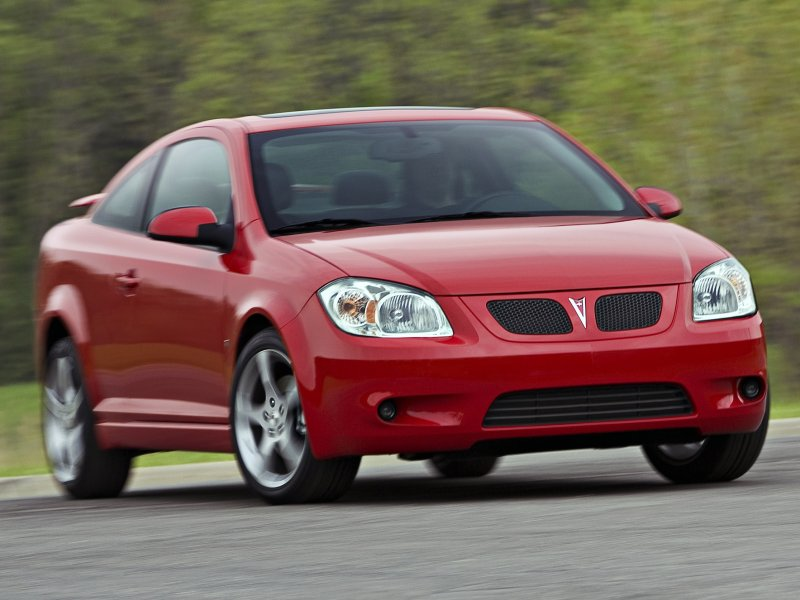
\includegraphics[scale=0.2]{\img/g5-quantize0.png}
\quad
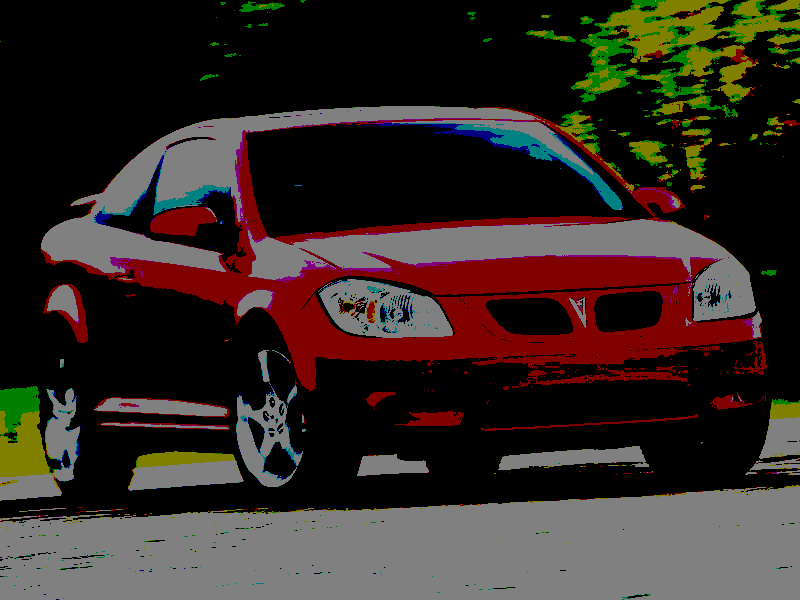
\includegraphics[scale=0.2]{\img/g5-quantize7.png}
\caption{A sporty coupe with quantization level 0 (left) and
level 7 (right).}
\label{fig:g5_quantize}
\end{figure}

Given an ordinary image of size $w \times h$ and a quantization level
$q$ between 0 and 7, inclusive, for each pixel in the image, take each
color component (red, green and blue) and clear the lowest $q$ bits.
For example, suppose the color components for a pixel are given by the
bytes
\begin{quote}
\renewcommand{\arraystretch}{1.2}
\begin{tabular}{lll}
   Red                  & Green                & Blue
\\\hline
   \lstinline'01101011' & \lstinline'10111110' & \lstinline'11010111'
\end{tabular}
\end{quote}
If the quantization level is 5, then the resulting pixel should have
the following color components (note how the lower 5 bits are all cleared to 0):
\begin{quote}
\renewcommand{\arraystretch}{1.2}
\begin{tabular}{lll}
   Red                  & Green                & Blue
\\\hline
   \lstinline'01100000' & \lstinline'10100000' & \lstinline'11000000'
\end{tabular}
\end{quote}
Note that an image processed with a quantization level of 0 should not change.
For each pixel, do not change its alpha component.




\vspace{0.1in}

\begin{task}[6]
\TAGS{array, correctness, safety, testing}
  Create a C0 file \lstinline'quantize.c0' with a function
  \lstinline'quantize' matching the following prototype:
\begin{lstlisting}
pixel_t[] quantize(pixel_t[] pixels, int width, int height, int q_level);
\end{lstlisting}
This function should implement the algorithm described above,
given an array \lstinline'pixels' representing an image of width
\lstinline'width' and height \lstinline'height' using a quantization
level \lstinline'q_level'.
\end{task}

We will compile your program as follows:
\begin{quote}
\begin{lstlisting}[language={[coin]C}]
% cc0 -d imageutil.c0 quantize.c0 quantize-main.c0 -o quantize
\end{lstlisting}
\end{quote}
using your \lstinline'imageutil.c0' and \lstinline'quantize.c0' files.
Your code must compile using these instructions with files shown in the order
given. Do NOT include a main function in your \lstinline'quantize.c0' file.
Sample usage is:
\begin{quote}
\begin{lstlisting}[language={[coin]C}]
% ./quantize -i images/g5.png -q 6
\end{lstlisting}
\end{quote}
Running this command should produce an image,
\lstinline'images/g5_quantize.png', that is identical to the file
\lstinline'images/g5-quantize6.png' distributed with the handout.


%%% Local Variables:
%%% mode: latex
%%% TeX-master: "main"
%%% End:
